\subsection{Ring configurations}

We have now seen that rings with nothing on their interior are already reducible. The natural next step would be to consider rings with an interior $\core$ called a \textit{core}. These will be called \textit{ring configurations}, since they are configurations with a ring as their boundary. All configurations used in the four color theorem are ring configurations!

\begin{definition}
    A planar graph $\confg = R_n + \core$ consisting of a ring $R_n$ and a \emph{core} $\core$ is called a \emph{ring configuration} on $R_n$.
\end{definition}

\begin{figure}[!h]
    \centering
        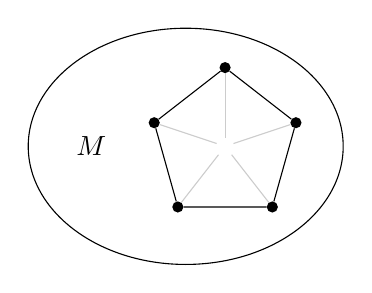
\begin{tikzpicture}
        \draw[fill=white] (-0.5, 0) ellipse (2cm and 1.5cm);
        %\draw[fill=lightgray, draw=black] (0,0) circle (1.25cm);
        %\draw[fill=white] (0,0) circle (0.75cm);
        \node at (-0.7, 0.9) {$\confg$};
        \node at (-1.7, 0) {$M$};

        \node[inner sep=1mm] (c) at (0, 0) {$\core$};
        \node[circle, fill, scale=0.015cm] (l1) at (0, 1) { };
        \node[circle, fill, scale=0.015cm] (l2) at (0.9, 0.30) { };
        \node[circle, fill, scale=0.015cm] (l3) at (0.6, -0.77) {};
        \node[circle, fill, scale=0.015cm] (l4) at (-0.6, -0.77) {};
        \node[circle, fill, scale=0.015cm] (l5) at (-0.9, 0.30) {};

        \draw[opacity=0.2] (c) -- (l1);
        \draw[opacity=0.2] (c) -- (l2);
        \draw[opacity=0.2] (c) -- (l3);
        \draw[opacity=0.2] (c) -- (l4);
        \draw[opacity=0.2] (c) -- (l5);
        \draw (l1) -- (l2) -- (l3) -- (l4) -- (l5) -- (l1);
    \end{tikzpicture}
    \caption{A graph $M+\confg$ with a ring configuration $\confg$ on $R_5$.}
\end{figure}

If a ring configuration $\confg$ on $R$ is contained in a graph $G$, then the ring $R$ acts as border between the interior $\core$ and exterior $M$. Suppose that we removed from $G$ the interior $\core$ of $\confg$ to obtain the graph $M+R$. If we colored $M+R$ and $\confg$ individually, then we could add the interior $\core$ back if the two colorings have the same colors on the ring $R$. This is the essence of $k$-reducibility. We prove that such a \textit{common ring coloring} can always be found. Mathematically, we phrase this as 

\begin{equation}
    \Phi(\confg) \;\cap\; \Phi(M+R) \quad \neq \quad\varnothing.
\end{equation}

I.e, the sets of possible ring colorings of $R$ in $\confg$ and $M+R$ have a common element. Given a configuration $\confg$, we can question whether such a common element exists for all graphs $M + \confg$. To answer this question, we must know to \textit{some} degree which colorings exist in $\Phi(M+R)$. Such colorings we  call \textit{guaranteed colorings}. They are all we can work with if the graph $M$ is arbitrary.


